\subsection{Interacting with the Data}
After having filtered and classified the data, the framework should provide a means for the client to interact with the resulting data. In this subsection, several ways to do so are compared, after which we decide which path to take.

\subsubsection{Query Language}

One possibility is to let the client query the data. For this, we designed a simple, easy to use query language specific to the domain of research. It has the following syntax:

\begin{center}
\begin{tabular}{ |c|c| } 
 \hline
 ! & Logical NOT operation \\
 \& & Logical AND operation \\ 
 $|$ & Logical OR operation \\ 
 $(~A~\&~B~)$ & Grouping of clauses \\
 $A > R > B$ & Relation R between cities A and B \\
 \hline
\end{tabular}
\end{center}

In figure \ref{fig:ql-example}, an example is shown that queries the "Shopping" relation between Rotterdam and Amsterdam and between Rotterdam and Den Haag.

\begin{figure}[ht]
\centering
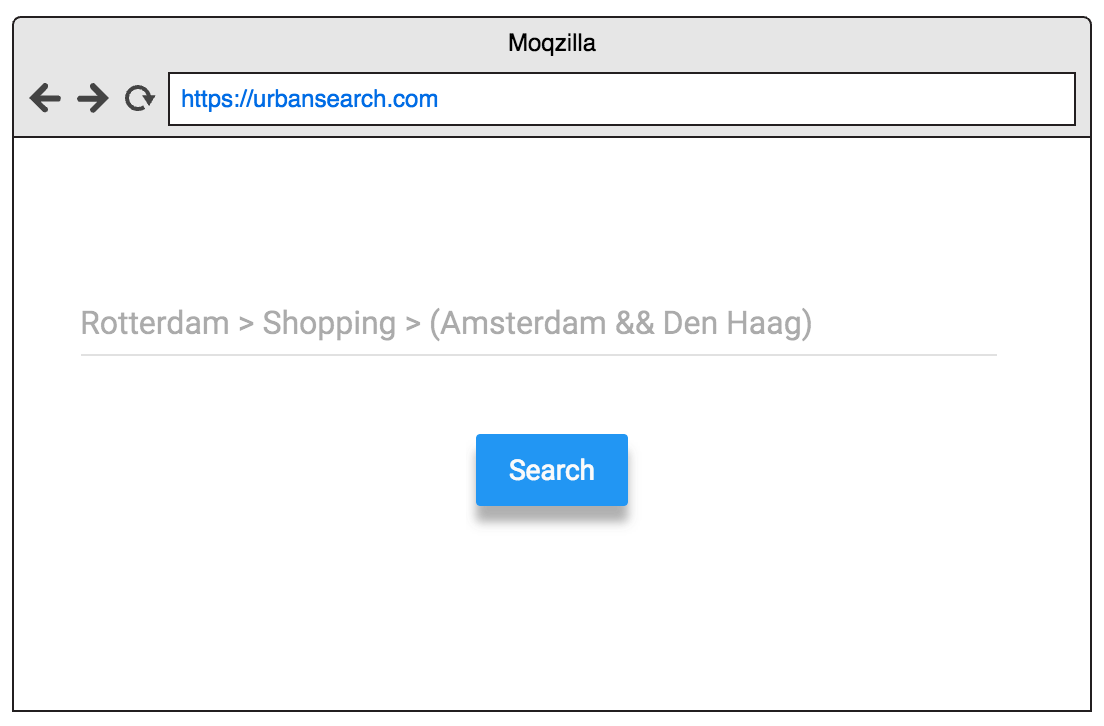
\includegraphics[width=0.75\textwidth]{ql-example}
\caption{Example interface for the query language}
\label{fig:ql-example}
\end{figure}

\subsubsection{Query Composer Interface}

Another possibility is to offer the client a query composition interface. This interface would have the same functionality as the previously mentioned query language, but is more intuitive to use for new users. An example of the interface is given in figure \ref{fig:qi-example}.

\begin{figure}[ht]
\centering
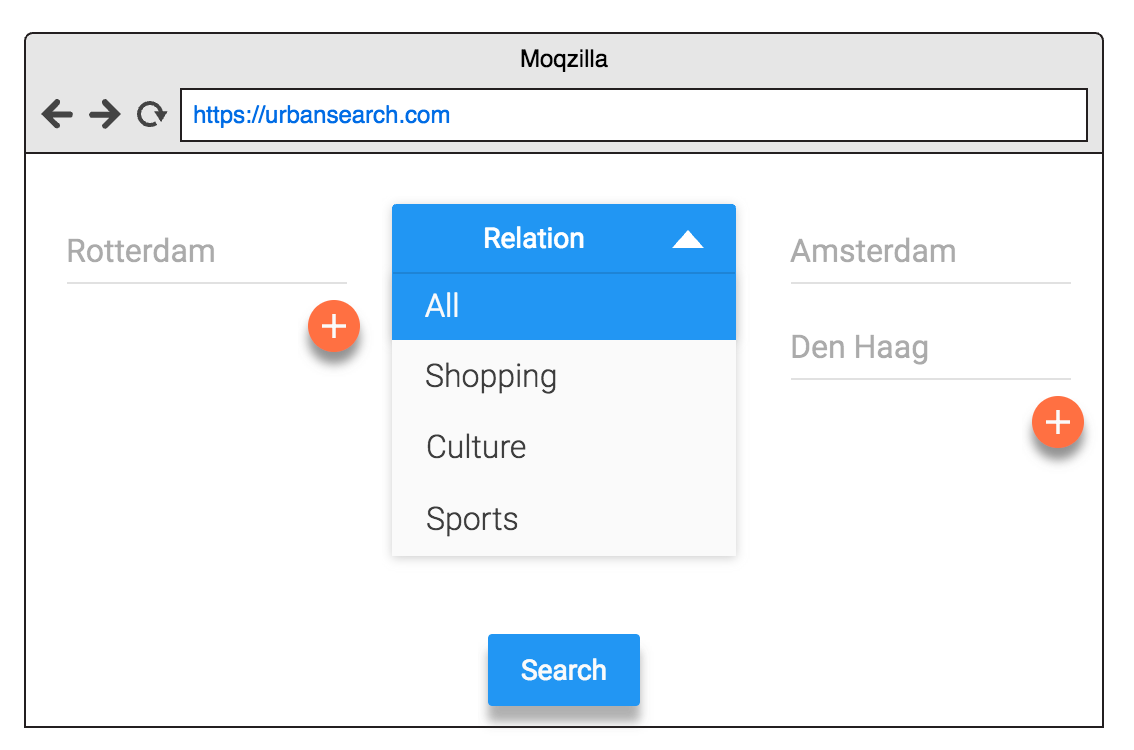
\includegraphics[width=0.75\textwidth]{qi-example}
\caption{Example interface for the query composer}
\label{fig:qi-example}
\end{figure}

\subsubsection{Interactive Search}

The last option we investigated is an interactive approach to querying data. For this, the client interacts with a map containing relations and cities. A very simple example is given in figure \ref{fig:ii-example}.

\begin{figure}[ht]
\centering
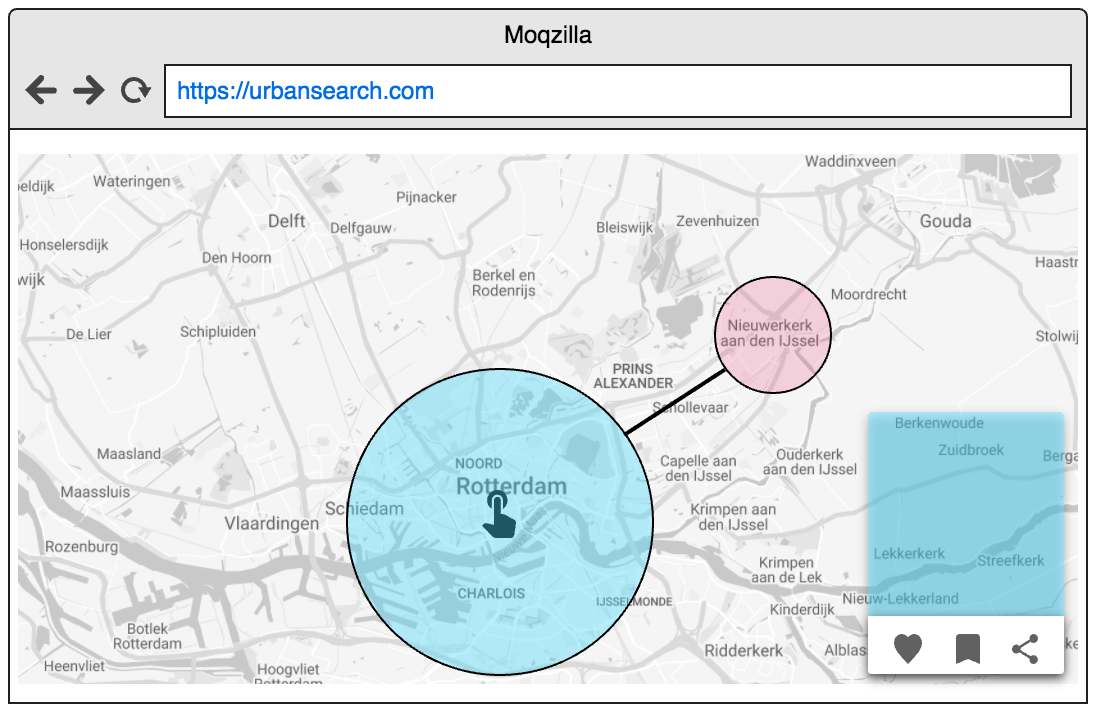
\includegraphics[width=0.75\textwidth]{ii-example}
\caption{Example of an interactive map}
\label{fig:ii-example}
\end{figure}

In this setup the user clicks on cities and relations on the map. This event triggers a query on the back-end and the resulting data is visualised on the map. An example of such an event is to show information about the selected city.

\subsubsection{Conclusion}

In association with the client, we conclude that the best option to go with is the interactive map.
This way, the client has easy access to the data and this pattern of interaction best suits the work flow that the client envisioned prior to the project. The creation of complex queries is also made a lot easier. The user does not have to write or compose a complex query in advance but can do it directly on the map. Thus, retrieving a visual representation of several cities, interconnected with multiple relations, only involves selecting cities and relations on the map. Interaction directly with the map also reduces the need to go to a separate page to compose a query. This speeds up the use of the system by reducing page loads and it interrupts the work flow of the user less.